\section{Training data acquistion protocol}

The inclusion citeria for the study was healthy and able bodied subjects. Four subjects (three men and one woman, ages:) participed in the training session. The subjects performed four different hand gestures: ulnar deviation, radial deviation, flexion and extension of the wrist, as shown in \figref{fig:handgest}. The order in execution of the movements was the same for each subject.

\begin{figure}[H]                    
	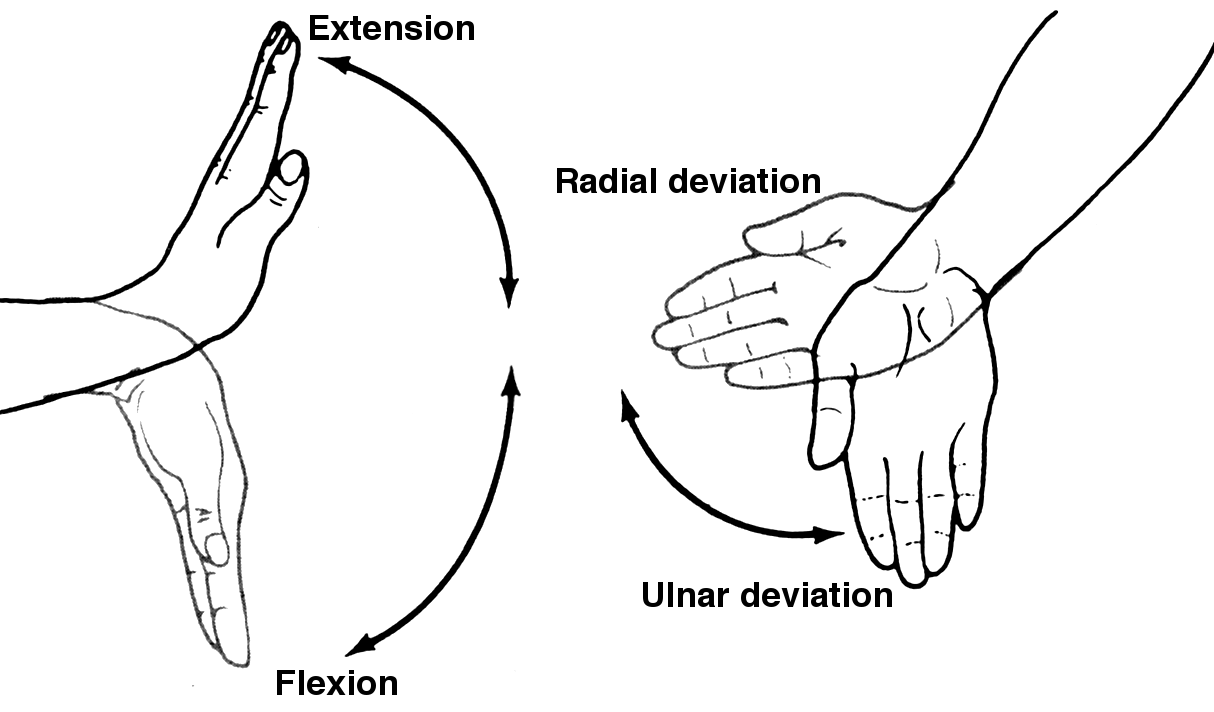
\includegraphics[width=.5\textwidth]{figures/Anatomy/wrist_move}  %<--but is not needed.
	\caption{Flexion, extension, radial and ulnar deviation of the hand. Modified from  \cite{hamilton2008}}
	\label{fig:handgest}  %<--give the figure a label, so you can reference!
\end{figure}

%In order to accomplish the study a Graphical User Interface $\left( GUI\right)$ had been created.The subjects of this study were familiar with the operation of the GUI.

Each hand gesture was performed as a fraction of the maximum voluntary contraction $\left( MVC\right)$ set as 25\% , 50\% and 75\%. The MVC reference was fixed as the highest values acquired from the four different hand gestures MVCs. The subjects performed the MVC of each gesture with two minues rest in between to avoid fatigue.

The acquisition of the fraction of each hand gesture consited of four chronologic phases: relaxed phase, transition phase, plateau phase and relaxed phase. This are depicted as a trapeze in a plot. In the performance of each gesture, EMG signals of the subject are represented as a dot in the trapeze window. The subject should follow the shape of the trapeze thought the dot as best as possible. The recording of the fraction of MVC of each gesture was ten seconds. The plateu phase, where the contraction is at its highest stage was four seconds.
  
The subjects were in a stand position during the data acquisition procedure. Due to the fact that the hand gestures only consists of wrist movements, the subjects should not move the fingers during the data aquisition. Hand gestures were performed in five different limb positions, illustrated in the figure \figref{fig:limbpos}.
%maybe change the limb positions
\begin{figure}[H]                    
	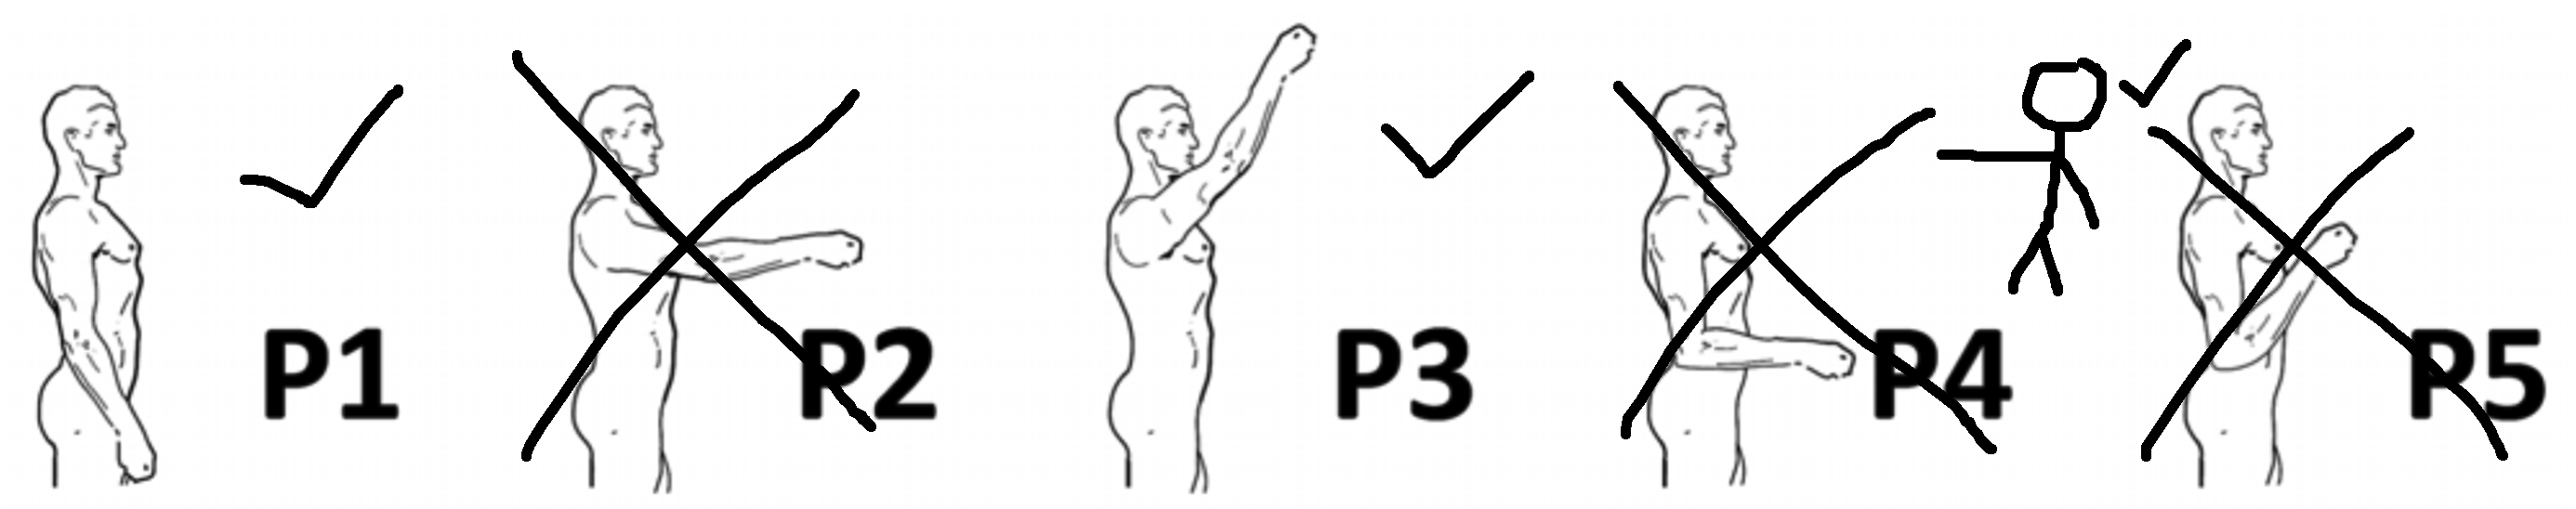
\includegraphics[width=1\textwidth]{figures/protocol/limb_position}  %<--but is not needed.
	\caption{Limb positions inspired from \cite{Fougner2011}}
	\label{fig:limbpos}  %<--give the figure a label, so you can reference!
\end{figure}

The limb positions consist of: 1.Relaxed arm hanging at side of torso, 2.Straight arm reaching horizontally forward, 3.Straight arm reaching up 45 degrees from vertical, 4.Humerus hanging at side, where forearm is horizontal and 5.Humerus hanging at side, where the forearm is 45 degrees above horizontal.

A relax time was given between trials in order to avoid shoulder fatigue.
%time of rest?

\begin{table}[h]
	\centering
\scalebox{.75}{
		\begin{tabular}{|l|l|l|l|l|l|}
		\hline
		& Limb 1 & Limb 2 & Limb 3 & Limb 4 & Limb 5 \\ \hline
		\begin{tabular}[c]{@{}l@{}}MVC\\ ulnar\end{tabular} & & & & & \\ \hline
		\begin{tabular}[c]{@{}l@{}}25 \%\\ ulnar\end{tabular} & & & & & \\ \hline
		\begin{tabular}[c]{@{}l@{}}50 \%\\ ulnar\end{tabular} & & & & & \\ \hline
		\begin{tabular}[c]{@{}l@{}}75 \%\\ ulnar\end{tabular} & & & & & \\ \hline
		\begin{tabular}[c]{@{}l@{}}MVC\\ radial\end{tabular} & & & & & \\ \hline
		\begin{tabular}[c]{@{}l@{}}25 \%\\ radial\end{tabular} & & & & & \\ \hline
		\begin{tabular}[c]{@{}l@{}}50 \%\\ radial\end{tabular} & & & & & \\ \hline
		\begin{tabular}[c]{@{}l@{}}75 \%\\ radial\end{tabular} & & & & & \\ \hline
		\begin{tabular}[c]{@{}l@{}}MVC\\ flex.\end{tabular} & & & & & \\ \hline
		\begin{tabular}[c]{@{}l@{}}25 \%\\ flex.\end{tabular} & & & & & \\ \hline
		\begin{tabular}[c]{@{}l@{}}50 \%\\ flex.\end{tabular} & & & & & \\ \hline
		\begin{tabular}[c]{@{}l@{}}75 \%\\ flex.\end{tabular} & & & & & \\ \hline
		\begin{tabular}[c]{@{}l@{}}MVC\\ ext.\end{tabular} & & & & & \\ \hline
		\begin{tabular}[c]{@{}l@{}}25 \%\\ flex.\end{tabular} & & & & & \\ \hline
		\begin{tabular}[c]{@{}l@{}}50 \%\\ flex.\end{tabular} & & & & & \\ \hline
		\begin{tabular}[c]{@{}l@{}}75 \%\\ flex.\end{tabular} & & & & & \\ \hline
		\begin{tabular}[c]{@{}l@{}}25 \%\\ ext.\end{tabular} & & & & & \\ \hline
		\begin{tabular}[c]{@{}l@{}}50 \%\\ ext.\end{tabular} & & & & & \\ \hline
		\begin{tabular}[c]{@{}l@{}}75 \%\\ ext.\end{tabular} & & & & & \\ \hline
	\end{tabular}}

	\caption{My caption}
	\label{my-label}
\end{table}
